\section{Case Study Results}
\label{sec:results}

In this section, we present the results of our case study with respect to our research questions.
For each research question, we present our approach and discuss the results.

\subsection*{(RQ1) \rqi}

\begin{figure}
  \centering
  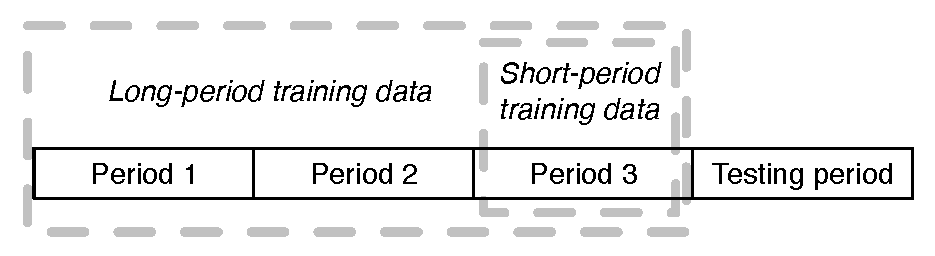
\includegraphics[width=0.9\columnwidth]{figures/period_examples.pdf}
  \caption{An illustrative example of the types of the JIT model types.}
  \label{fig:period_ex}
\end{figure}

\begin{figure*}[t]
  \centering
  \subfloat[AUC in three-month periods ({\sc Qt})]{
    \includegraphics[width=0.88\columnwidth]{figures/perf/qt_lrm_4_AUC.pdf}
    \label{fig:perf_qt_auc}
  }
  \subfloat[AUC in six-month periods ({\sc Qt})]{
    \includegraphics[width=0.88\columnwidth]{figures/perf/qt_lrm_2_AUC.pdf}
    \label{fig:six_perf_qt_auc}
  }
  \qquad
  \subfloat[AUC in three-month periods ({\sc OpenStack})]{
    \includegraphics[width=0.88\columnwidth]{figures/perf/openstack_lrm_4_AUC.pdf}
    \label{fig:perf_openstack_auc}
  }
  \subfloat[AUC in six-month periods ({\sc OpenStack})]{
    \includegraphics[width=0.88\columnwidth]{figures/perf/openstack_lrm_2_AUC.pdf}
    \label{fig:six_perf_openstack_auc}
  }
  \qquad
  \subfloat[Brier score in three-month periods ({\sc Qt})]{
    \includegraphics[width=0.88\columnwidth]{figures/perf/qt_lrm_4_Brier.pdf}
    \label{fig:perf_qt_brier}
  }
  \subfloat[Brier score in six-month periods ({\sc Qt})]{%
    \includegraphics[width=0.88\columnwidth]{figures/perf/qt_lrm_2_Brier.pdf}
    \label{fig:six_perf_qt_brier}
  }
  \qquad
  \subfloat[Brier score in three-month periods ({\sc Openstack})]{
    \includegraphics[width=0.88\columnwidth]{figures/perf/openstack_lrm_4_Brier.pdf}
    \label{fig:perf_openstack_brier}
  }
  \subfloat[Brier score in six-month periods ({\sc OpenStack})]{%
    \includegraphics[width=0.88\columnwidth]{figures/perf/openstack_lrm_2_Brier.pdf}
    \label{fig:six_perf_openstack_brier}
  }
  \caption{The predictive performance of JIT models as the studied systems age.}
  \label{fig:perf}
\end{figure*}

\begin{figure*}[t]
  \centering
  \subfloat[AUC in three-month periods ({\sc Qt})]{
    \includegraphics[width=0.88\columnwidth]{figures/perf/qt_lrm_4_AUC_delta.pdf}
    \label{fig:perf_qt_auc_delta}
  }
  \subfloat[AUC in six-month periods ({\sc Qt})]{
    \includegraphics[width=0.88\columnwidth]{figures/perf/qt_lrm_2_AUC_delta.pdf}
    \label{fig:six_perf_qt_auc_delta}
  }
  \qquad
  \subfloat[AUC in three-month periods ({\sc OpenStack})]{%
    \includegraphics[width=0.88\columnwidth]{figures/perf/openstack_lrm_4_AUC_delta.pdf}
    \label{fig:perf_openstack_auc_delta}
  }
  \subfloat[AUC in six-month periods ({\sc OpenStack})]{%
    \includegraphics[width=0.88\columnwidth]{figures/perf/openstack_lrm_2_AUC_delta.pdf}
    \label{fig:six_perf_openstack_auc_delta}
  }
  \qquad
  \subfloat[Brier score in three-month periods ({\sc Qt})]{
    \includegraphics[width=0.88\columnwidth]{figures/perf/qt_lrm_4_Brier_delta.pdf}
    \label{fig:perf_qt_brier_delta}
  }
  \subfloat[Brier score in six-month periods ({\sc Qt})]{
    \includegraphics[width=0.88\columnwidth]{figures/perf/qt_lrm_2_Brier_delta.pdf}
    \label{fig:six_perf_qt_brier_delta}
  }
  \qquad
  \subfloat[Brier score in three-month periods ({\sc OpenStack})]{%
    \includegraphics[width=0.88\columnwidth]{figures/perf/openstack_lrm_4_Brier_delta.pdf}
    \label{fig:perf_openstack_brier_delta}
  }
  \subfloat[Brier score in six-month periods ({\sc OpenStack})]{%
    \includegraphics[width=0.88\columnwidth]{figures/perf/openstack_lrm_2_Brier_delta.pdf}
    \label{fig:six_perf_openstack_brier_delta}
  }
  \caption{The delta in the estimated performance of JIT models as the studied systems age.}
  \label{fig:perf_delta}
\end{figure*}

\smallsection{RQ1: Approach}
To address RQ1, we study how quickly a JIT model loses its predictive power by training JIT models for each of the time periods (i.e., varying the training period), and measuring their performance on future periods.
As illustrated in Figure~\ref{fig:period_ex}, for each period, we train two types of models:

\begin{enumerate}
  \item \underline{\bf Short-period models} are JIT models that are only trained using changes that occurred during one time period.
    We train short-period models because older changes may have characteristics that no longer apply to the latest changes.
  \item \underline{\bf Long-period models} are JIT models that are trained using all of the changes that occurred during or prior to a particular period.
    We train long-period models because recent work suggests that larger amounts of training data tend to yield defect models that perform better, even when biases are introduced~\cite{rahman2013fse}.
    Hence, despite potential changes in the properties of fix-inducing changes, being exposed to additional data may improve the performance of our JIT models.
\end{enumerate}

After training our JIT models, we test their performance when they are applied to the periods that occur after the last training period.
As described in Section~\ref{sec:ma}, we measure the performance of our models using the AUC (discriminatory power) and the Brier score (calibration).

For example, Figure~\ref{fig:period_ex} illustrates that for a training period 3, the short-period model is trained using the changes that occurred during period 3, while the long-period model is trained using changes that occurred during periods 1, 2, and 3.
These short-period and long-period models of period 3 are tested using periods 4 through to the last studied period.
The AUC and Brier performance scores are computed for each testing period individually.

Finally, we plot the trends in AUC and Brier performance scores over time using heatmaps.
In Figure~\ref{fig:perf}, the shade of a box indicates the performance value, where blue shades indicate strong performance, red shades indicate weak performance, and the palest (white) shade indicates the performance that a random guessing model would achieve (on average).
In Figure~\ref{fig:perf_delta}, the shade indicates the difference in AUC and Brier performance scores between the training and testing periods in question.
Red, blue, and pale (white) shades indicate drops, improvements, and unchanged performance in the testing period, respectively.

\smallsection{RQ1: Results}
\textbf{Models that are trained using periods that are closer to the testing period tend to outperform models that are trained using older periods.}
When we focus on the columns of Figure~\ref{fig:perf}, the performance values tend to improve as the training period increases.
In {\sc Qt}, the trend is especially prominent in testing periods 5 and later of the three-month period models, where at least one year has elapsed.
For example, the long-period sections of Figures~\ref{fig:perf_qt_auc} and~\ref{fig:perf_openstack_auc} show an AUC score improvement of 16--24 percentage points for {\sc Qt} and 6--12 percentage points for {\sc OpenStack} by training using the most recent data (i.e., the period just prior to the testing period) instead of the data from period 1.
Figures~\ref{fig:perf_qt_brier} and~\ref{fig:perf_openstack_brier} also show a boost in Brier score of 12--28 and 6--7 percentage points for {\sc Qt} and {\sc OpenStack}, respectively.

Although the magnitude is lower, similar improvement trends are observed in the six-month periods.
Figures~\ref{fig:six_perf_qt_auc} and~\ref{fig:six_perf_openstack_auc} show an AUC score improvement of 5--6 percentage points in {\sc Qt} and 9 percentage points in {\sc OpenStack}.
While Figure~\ref{fig:perf_qt_brier} shows an improvement in Brier score of only 1 percentage point for {\sc Qt}, Figure~\ref{fig:perf_openstack_brier} shows a boost of 5 percentage points for {\sc OpenStack}.

The improving trend tends to stabilize (at least) one period before the testing period.
For example, Figures~\ref{fig:perf_qt_auc} and~\ref{fig:perf_openstack_auc} show that the AUC improvement gained by adding the most recent three-month period to the long-period models of both studied systems is -1--2 percentage points.
The -1 indicates a 1 percentage point loss in testing periods 6 and 8 of {\sc Qt} (0.68 and 0.67 in training periods 4 and 5) and {\sc OpenStack} (0.64 and 0.63 in training periods 5 and 6), respectively.
Figures~\ref{fig:six_perf_qt_auc} and~\ref{fig:six_perf_openstack_auc} show similar trends of adding the most recent six-month period to the long-period models of both studied systems yields improvements of 0--3 percentage points.
Figures~\ref{fig:perf_qt_brier},~\ref{fig:six_perf_qt_brier},~\ref{fig:perf_openstack_brier}, and~\ref{fig:six_perf_openstack_brier} show similar fluctuations of 0--2 percentage points in Brier score.

\textbf{Our models lose a large amount of predictive power one year after being trained.}
Analysis of the rows of Figure~\ref{fig:perf_delta} shows that after one year, there is often a large drop in the AUC and a sharp increase in the Brier score.
Figures~\ref{fig:perf_qt_auc_delta} and~\ref{fig:perf_openstack_auc_delta} show that our short-period models lose 3--22 and 3--34 AUC percentage points one year after being trained (i.e., $\textit{testing period} = \textit{training period} + 4$) in {\sc Qt} and {\sc OpenStack}, respectively.
The drops of only three AUC percentage points are observed in period 7 of {\sc Qt} and period 9 of {\sc OpenStack}, which Figures~\ref{fig:perf_qt_auc} and~\ref{fig:perf_openstack_auc} show have a tendency to yield strong performance scores (with performance scores noticeably higher than those of nearby rows).
If those periods are omitted, the drops in AUC associated with our short-period models range from 11--22 percentage points in {\sc Qt} and 14--34 percentage points in {\sc OpenStack}.
Moreover, while training periods 1 and 2 of the long-period models in {\sc Qt} also suffer from large AUC drops of 22 and 13 percentage points, respectively, our long-period models that we train using periods 5 and later tend to retain their predictive power, only losing 1--9 AUC percentage points after one year.
Similarly, after one year, the Brier score of our {\sc Qt} and {\sc OpenStack} models drop by up to 11 and 19 percentage points, respectively (see Figures~\ref{fig:perf_qt_brier_delta} and \ref{fig:perf_openstack_brier_delta}).


Interestingly, Figures~\ref{fig:perf_qt_auc_delta},~\ref{fig:six_perf_qt_auc_delta},~\ref{fig:perf_qt_brier_delta}, and~\ref{fig:six_perf_openstack_brier_delta} show that after losing a large amount of predictive power after one year, our {\sc Qt} and {\sc OpenStack} models of periods 1 and 2 recover some predictive power in later periods.
This suggests that the properties of fix-inducing changes in those later periods share some similarities with the fix-inducing changes of the earliest periods.
We investigate this in RQ2.

\textbf{Long-period JIT models do not always retain predictive power for longer than short-period JIT models.}
Note that the short-period and long-period models for period 1 are identical because there is no additional data added when training the long-period model.
Hence, we only discuss the improvement in retention of predictive power for the JIT models that are trained using periods 2 and later.

We observe improvements in the predictive power of our {\sc Qt} models when they are tested in both the three-month and six-month settings.
The rows of Figures~\ref{fig:perf_qt_auc_delta} and~\ref{fig:six_perf_qt_auc_delta} show that the long-period models of periods 2 and later retain more predictive power than their short-period counterparts in terms of AUC.
For example, Figure~\ref{fig:perf_qt_auc_delta} shows that the short-period model that was trained using period 3 drops 8 percentage points in AUC when it is tested on period 4, while the long-period model only drops 5 percentage points under the same circumstances.
Moreover, Figure~\ref{fig:six_perf_qt_auc_delta} shows that long-period models in the six-month period setting drop at most 3 percentage points of AUC when they are tested on the final period (period 6), while short-period models drop up to 10 percentage points.
Figures~\ref{fig:perf_qt_brier_delta} and~\ref{fig:six_perf_qt_brier_delta} show that there is also an improvement in the retention of Brier score for {\sc Qt}.

Surprisingly, in {\sc OpenStack}, Figures~\ref{fig:perf_openstack_auc_delta} and~\ref{fig:perf_openstack_brier_delta} show
 that the long-period models underperform with respect to the short-period models in terms of AUC and Brier score.
 This suggests that fix-inducing changes vary from period to period, with a sensitivity to more recent changes being more beneficial than accruing additional data in {\sc OpenStack}.

\conclusionbox{A large proportion of the predictive power of JIT models is lost one year after being trained, suggesting that properties of fix-inducing changes may be in flux. JIT performance decay can be dampened by training JIT models using data that is recorded nearer to the testing period (i.e., more recent data).}

\subsection*{(RQ2) \rqii}

\smallsection{RQ2: Approach}
In order to address RQ2, we compute the normalized Wald $\chi^2$ importance scores (see Section~\ref{sec:ma}) of each studied family of code change properties in each of our short-period and long-period JIT models.
We study trends in the importance scores using heatmaps.
The darker the shade of a given box, the more important that that family is to our model fit for that period.
Figure~\ref{fig:importance} shows the results of our family importance analysis.
In addition, we compute the p-values that are associated with the importance scores and denote the significance of each cell using asterisks (*).

\smallsection{RQ2: Results}
\textbf{The Size family is a consistent top-contributor to the fits of our models.}
Figure~\ref{fig:importance} shows that Size is often the most darkly shaded cell per period (columns).
Figures~\ref{fig:importance_qt} and~\ref{fig:six_importance_qt} show that in {\sc Qt}, the Size family accounts for 23\%--38\% and 23\%--37\% of the explanatory power of our three- and six-month long-period JIT models, respectively.
Moreover, Size accounts for 10\%--43\% and 13\%--37\% of the explanatory power of our three- and six-month short-period JIT models, respectively.
Figures~\ref{fig:importance_qt} and~\ref{fig:six_importance_qt} also show that the Size family is the top contributor in 8 of the 11 three-month periods and 5 of the 6 six-month periods of our short-period JIT models, and all of the three- and six-month periods for our long-period JIT models.
The contributed explanatory power of the Size family is statistically significant in all of the periods for our short- and long-period models in both three- and six-month settings ($p < 0.05$ and $p < 0.01$, respectively).

Similarly, Figures~\ref{fig:importance_openstack} and~\ref{fig:six_importance_openstack} show that in {\sc OpenStack}, the Size family accounts for 11\%--37\% and 15\%--19\% of the explanatory power of our three- and six-month long-period JIT models, respectively. 
Size also contributes 3\%--37\% and 14\%--25\% of the explanatory power of our three- and six-month short-period JIT models, respectively.
Moreover, Size is only a non-significant contributor to two of the nine three-month short-period models, providing a significant amount of explanatory power to all of the other three-month short- and long-period models, as well as all of the six-month short- and long-period models.
In short, the magnitude and consistency of the importance of Size suggests that advice about limiting change size is sound.

\begin{figure*}[t]
  \centering
  \subfloat[Three-month periods ({\sc Qt})]{
    \includegraphics[width=0.95\columnwidth]{figures/importance/qt_lrm_4.pdf}
    \label{fig:importance_qt}
  }
  \subfloat[Six-month periods ({\sc Qt})]{
    \includegraphics[width=0.95\columnwidth]{figures/importance/qt_lrm_2.pdf}
    \label{fig:six_importance_qt}
  }
  \qquad
  \subfloat[Three-month periods ({\sc OpenStack})]{%
    \includegraphics[width=0.95\columnwidth]{figures/importance/openstack_lrm_4.pdf}
    \label{fig:importance_openstack}
  }
  \subfloat[Six-month periods ({\sc OpenStack})]{%
    \includegraphics[width=0.95\columnwidth]{figures/importance/openstack_lrm_2.pdf}
    \label{fig:six_importance_openstack}
  }
  \caption{How the importance scores of the studied families of code change properties change over time. Shade indicates magnitude while asterisks indicate significance according to Wald $\chi^2$ test, where: * $p < 0.05$; ** $p < 0.01$; *** $p < 0.001$.}
  \label{fig:importance}
\end{figure*}

While the explanatory power of the Size family often dominates our models, there are periods where other families have larger importance scores.
For example, Figures~\ref{fig:importance_openstack} and~\ref{fig:six_importance_openstack} also show that in {\sc OpenStack}, the Review family achieves a larger importance score than the Size family in:
(a) periods 2, 3, and 6 of the three-month short-term models,
(b) periods 2--7 of the three-month long-period models,
(c) periods 1--3 of the six-month short-term models,
and (d) all periods of the six-month long-term models.
Figures~\ref{fig:importance_qt} shows that in {\sc Qt}, the Review family achieves a larger importance score than the Size family in periods 5, 6, and 9 of the three-month short-term models, while the History family achieves a larger importance score than the Size family in the short-period model of period 6.

\textbf{Fluctuations in family importance are common in short-period models.}
Figure~\ref{fig:importance} shows that the shades of family importance (rows) vary more in short-period models than they do in long-period models.
For example, in the three-month periods of {\sc Qt} (Figure~\ref{fig:importance_qt}), the delta of the maximum and minimum explanatory power in the Size family is 0.33 ($0.43 - 0.10$) and 0.15 ($0.38 - 0.23$) in the short- and long-period settings, respectively.
This is as one might expect, given that long-period models are eventually trained using much more data.
Nonetheless, varying family importance in short-period models is another indication of fluctuation of the properties of fix-inducing changes.

Fluctuations in family importance also do occur in long-period models, albeit less often than short-period models.
For example, Figure~\ref{fig:importance_openstack} shows that Diffusion, Reviewer Experience, and Review importance scores grow and shrink over the studied periods.
Reviewer Experience increases and decreases in importance as {\sc OpenStack} ages, while the importance of the Reviewer Experience and Diffusion fades in the early periods and grows again in later periods.

\textbf{Our awareness measures do not contribute a significant amount of explanatory power.}
In this paper, we propose author and reviewer awareness---two new code change properties that compute how much of the prior change activity the author and reviewer has been involved with (see Table~\ref{tab:metrics}).
Analysis of our model fits reveals that the awareness change properties did not improve our fits to a statistically significant degree.
In fact, author awareness is often highly correlated with other Experience properties, suggesting that in the studied systems, author awareness does not provide any new information that existing Experience measures do not already capture.
Despite the negative outcome of this empirical analysis, it may still be worthwhile to compute awareness values in future studies, since larger amounts of data may provide an opportunity for awareness values to differ from those of other Experience measures.

\conclusionbox{The importance of most families of code change properties fluctuate from period to period, suggesting that the properties of fix-inducing changes tend to evolve as projects age.}

\subsection*{(RQ3) \rqiii}

\begin{figure*}[t]
  \centering
  \subfloat[Three-month periods ({\sc Qt})]{
    \includegraphics[width=0.7\textwidth]{figures/stability/qt_lrm_4.pdf}
    \label{fig:stability_qt}
  }
  \subfloat[Six-month periods ({\sc Qt})]{
    \includegraphics[width=0.3\textwidth]{figures/stability/qt_lrm_2.pdf}
    \label{fig:six_stability_qt}
  }
  \vspace{-2mm}
  \qquad
  \subfloat[Three-month periods ({\sc OpenStack})]{%
    \includegraphics[width=0.7\textwidth]{figures/stability/openstack_lrm_4.pdf}
    \label{fig:stability_openstack}
  }
  \subfloat[Six-month periods ({\sc OpenStack})]{%
    \includegraphics[width=0.3\textwidth]{figures/stability/openstack_lrm_2.pdf}
    \label{fig:six_stability_openstack}
  }
  \caption{The stability of the importance scores of the studied families of code change properties over time ($\textit{FISDiff}(f,i,j)$).}
  \label{fig:stability}
\end{figure*}

\smallsection{RQ3: Approach}
To address RQ3, we study the stability of the importance scores of the studied families of code change properties.
To do so, we first select the short-period and long-period JIT models that we trained using each of the time periods.
For each model, we compute the Family Importance Score ($\textit{FIS}$) for each family $f$ in:
(a) the training period $i$ ($\textit{FIS}(f,i)$) and
(b) the short-period JIT models in each period $j$ in the year that follows after the training period (i.e., $\textit{FIS}(f,j)$, where $j \in \{i+1, i+2, \cdots, i+\textit{\# periods per year}\}$)).
The $\textit{FIS}(f,n)$ is the jointly tested model terms for all of the metrics belonging to a family $f$ in the model of period $n$.
Note that when computing $\textit{FIS}(f,j)$ (i.e., those values that belong to ``future'' time periods), we use short-period JIT models instead of long-period models because short-period models should more accurately reflect the characteristics of the period in question.
We then compute the differences between the importance scores in periods $i$ and $j$ using $\textit{FISDiff}(f,i,j) = \textit{FIS}(f,i) - \textit{FIS}(f,j)$.

It is important to note that $\textit{FISDiff}(f,i,j) > 0$ indicates that the importance of family $f$ is larger in period $i$ (the training period) than it is in period $j$, i.e., the JIT model that is trained using period $i$ {\em overestimates} the future importance of family $f$.
In these situations, quality improvement plans that are based on the importance of $f$ at the end of period $i$ would have a smaller impact than anticipated.

On the other hand, $\textit{FISDiff}(f,i,j) < 0$ indicates that the importance of family $f$ is smaller in period $i$ than it is in period $j$, i.e., the JIT model that is trained using period $i$ {\em underestimates} the importance of family $f$.
In these situations, quality improvement plans that are based on the importance of $f$ in period $i$ may miss important families that would yield larger quality improvements than anticipated.

Similar to RQ2, we show the $\textit{FISDiff}(f,i,j)$ values using heatmaps.
We also compute the p-values that are associated with the importance score of the model of period $i$, since this is the model upon which quality improvement plans would be based.
We again denote the statistical significance of these importance scores using asterisks (*).
For presentation clarity, we only show $\textit{FISDiff}(f,i,j)$ values for the year that follows the training of each model.
As shown below, this one-year period is enough to demonstrate interesting trends.

\smallsection{RQ3: Results}
{\textbf{Long-period models should be preferred for quality improvement planning.}
The short-period models of Figure~\ref{fig:importance} show several periods where trends in importance fluctuate sporadically.
These spikes and troughs in importance scores can have a misleading impact on quality improvement plans when they are the source of data that is used to train JIT models.
Figure~\ref{fig:stability} shows that long-period models tend to cope with these periods of sporadic fluctuation more gracefully than short-period models do.

For example, Figure~\ref{fig:importance_qt} shows that the Size family has a large spike in importance in period 7 of the three-month setting of {\sc Qt}.
Training periods 5 and 6 of Figure~\ref{fig:stability_qt} show that the importance of the Size family is underestimated by 18 and 22 percentage points, respectively for testing period 7 in short-period models.
Since the long-period models have a smoothing effect, these underestimates drop to 7 and 9 percentage points, respectively.
When period 7 becomes the training period in Figure~\ref{fig:stability_qt}, the impact of the Size family is overestimated by up to 23 percentage points in the short-period models.
The maximum overestimate for the related long-period models is 15 percentage points.

Turning to {\sc OpenStack}, Figure~\ref{fig:importance_openstack} shows that the Review family has a large spike in importance in period 6.
Training periods 4 and 5 of Figure~\ref{fig:stability_openstack} show that the importance of the Review family is underestimated by 57 and 46 percentage points, respectively in the short-period models.
Again, the smoothing effect of the long-period reduces the impact of this spike to 27 and 29 percentage points, respectively.

The six-month setting (Figures~\ref{fig:six_stability_qt} and~\ref{fig:six_stability_openstack}) shows less severe over/underestimates, also suggesting that larger amounts of training data will smooth the impact of period-specific fluctuations on quality improvement plans.

\textbf{The stability of many families of code change properties is project-sensitive.}
For example, the consistency of blue-shaded cells in Figure~\ref{fig:stability_qt} indicates that the importance of the Size family is often overestimated in {\sc Qt} (median of 5\%), especially in training period 2.
Indeed, Figure~\ref{fig:importance_qt} shows that importance of Size was largest at training period 2 of {\sc Qt}, trending downwards after that.
Conversely, the consistency of red-shaded cells in Figure~\ref{fig:stability_openstack} indicates that the importance of the Size family is often underestimated in {\sc OpenStack} (median of 2\%), especially in training periods 2 and 3.
Again, Figure~\ref{fig:importance_openstack} shows that importance of Size is growing as {\sc OpenStack} ages from period 2 and 3.
Models that are trained using the early periods tend to underestimate the importance of the Size family in later periods.

Similarly, Figure~\ref{fig:stability_qt} shows that the History family tends to be underestimated in {\sc Qt} (13 out of 24 periods for short-period and 20 out of 24 periods for long-period), while Figure~\ref{fig:stability_openstack} shows that the Review family tends to be overvalued in {\sc OpenStack} (17 out of 20 periods for short-period and 19 out of 20 periods for long-period).
Indeed, Figure~\ref{fig:importance_qt} shows that the History family tends to grow more important as {\sc Qt} ages, while Figure~\ref{fig:importance_openstack} shows that the Review family tends to become less important as {\sc OpenStack} ages.

%\todo{Diffusion, Rev. Exp, Review are not discussed.}

\conclusionbox{When constructing quality improvement plans, one should favour large caches of data (e.g., long-period models, six-month periods).
The importance of impactful families of code change properties like Size and Review are consistently under/overestimated in the studied systems.}
